\section{Solution approach}
    Give a brief description about the solution
    \pagebreak

  \section{Object Oriented Design}
    \subsection{Sequence Diagram}
      \vspace{1cm}
      \begin{figure}[h!]
        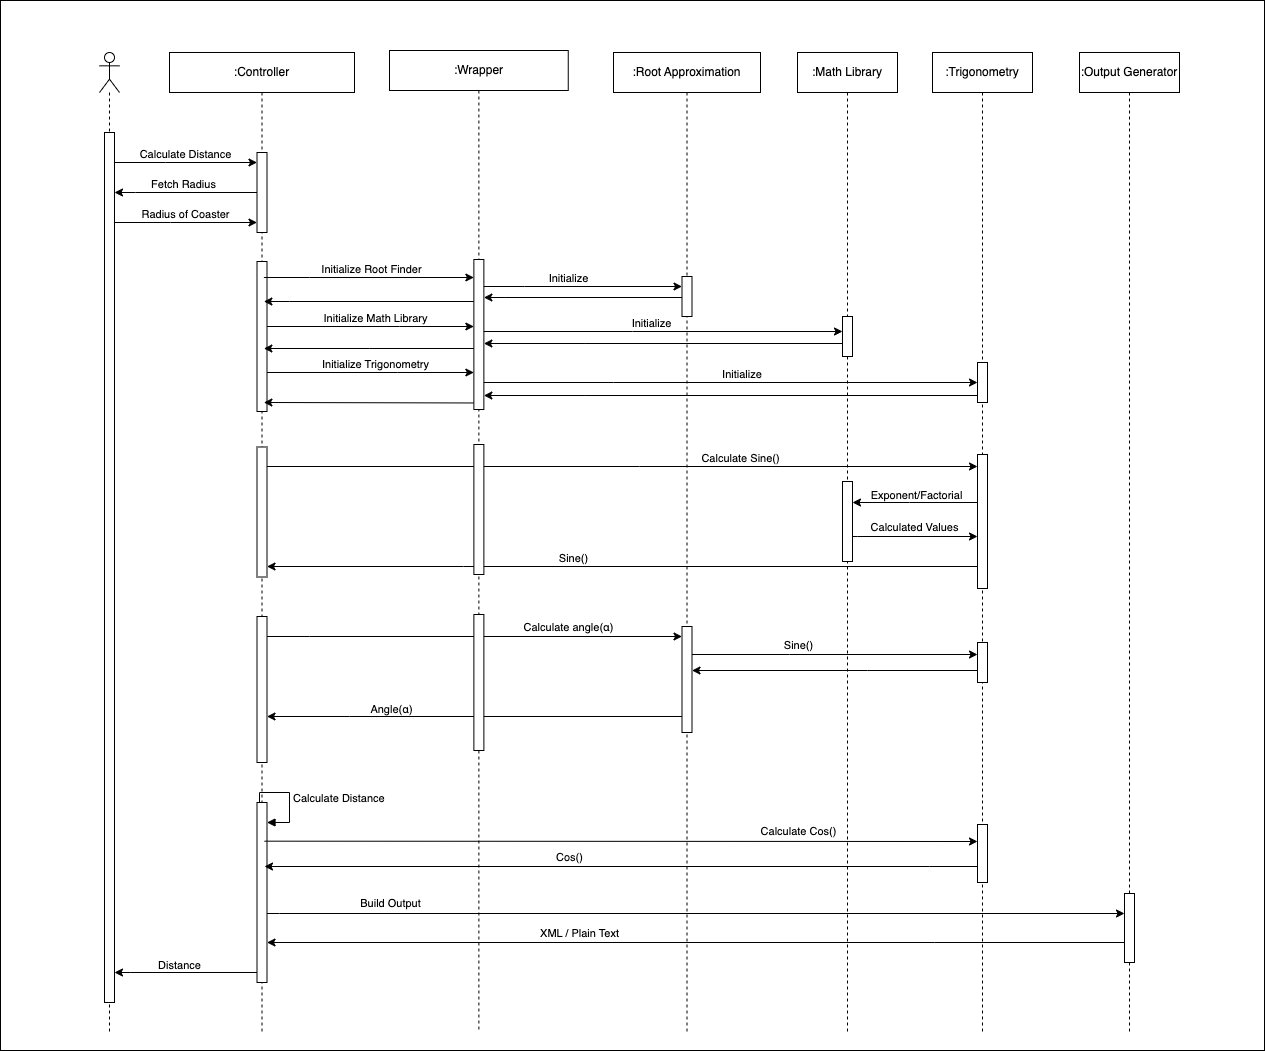
\includegraphics[width=1\linewidth]{resources/cheers-sequence.png}
        \vspace{.5cm}
        \caption{Flow of events for calculating distance}
        \label{fig:Sequence Diagram}
      \end{figure}
      \pagebreak

  \subsection{CRC Cards}
  \begin{figure}[h!]
      \centering
      \begin{tabular}{@{}c@{}}
        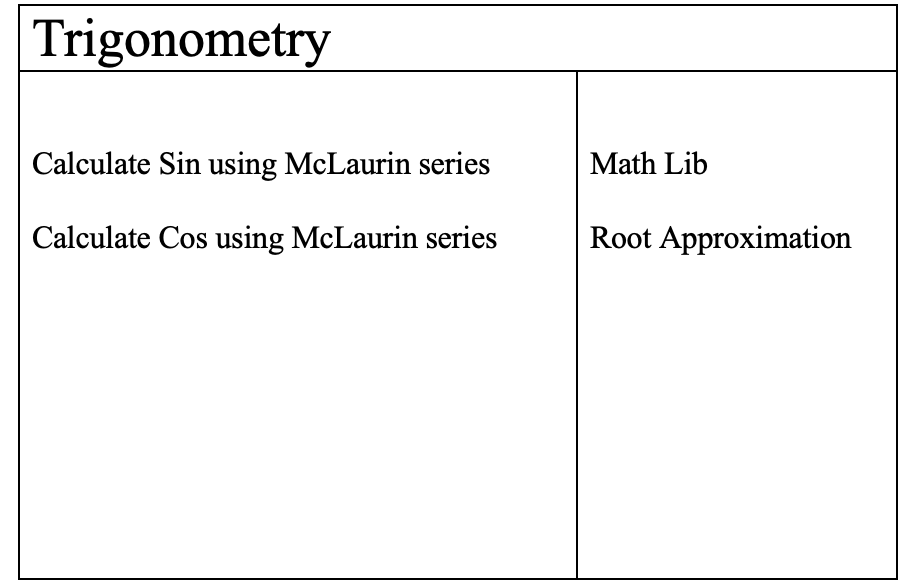
\includegraphics[width=.3\linewidth]{resources/Trigonometry.png} 
          \hspace*{30pt}
        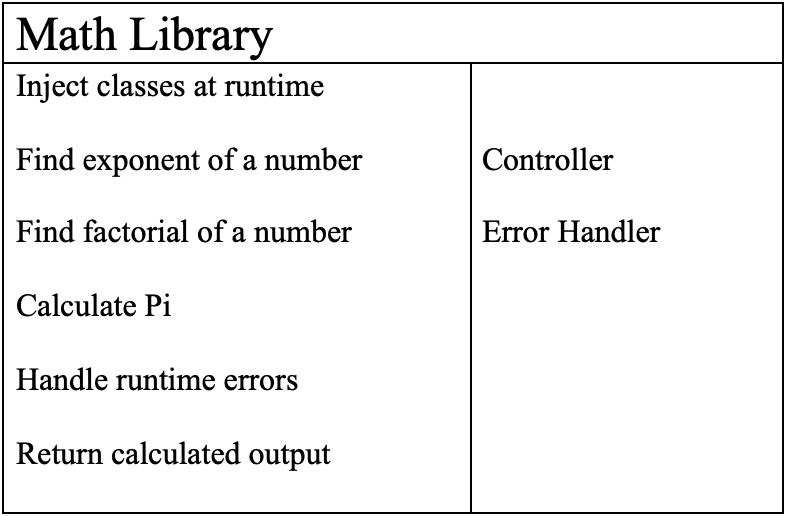
\includegraphics[width=.3\linewidth]{resources/MathLib.png}
      \end{tabular}
    
      \begin{tabular}{@{}c@{}}
          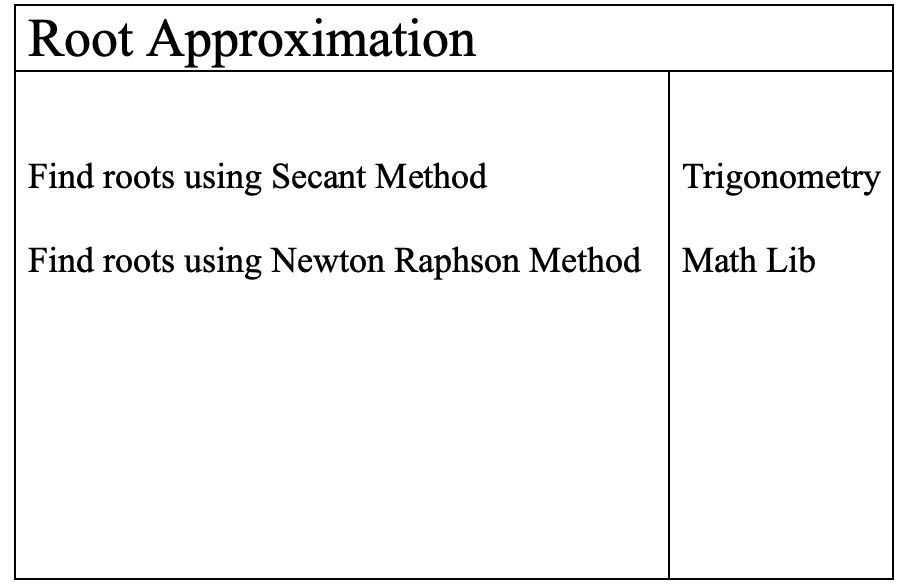
\includegraphics[width=.3\linewidth]{resources/RootApproximation.png} 
            \hspace*{30pt}
          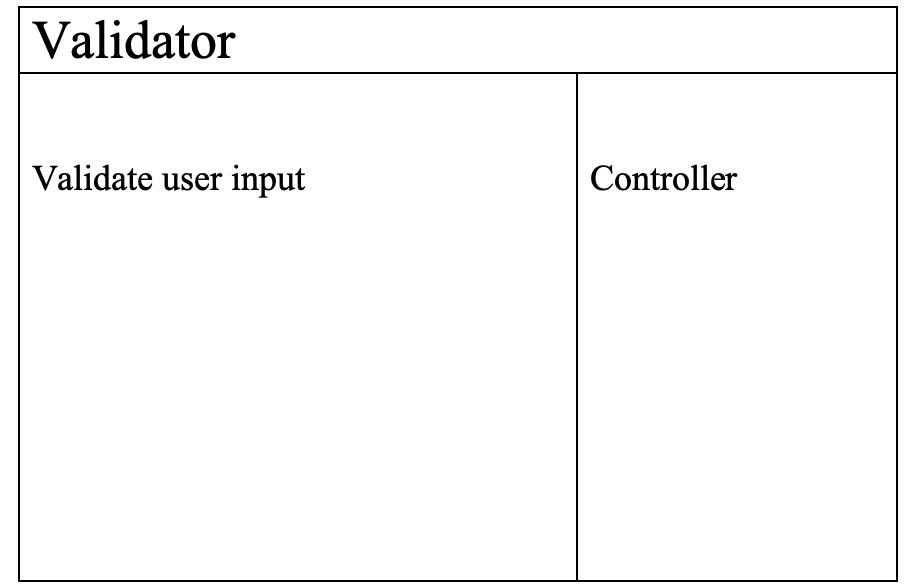
\includegraphics[width=.3\linewidth]{resources/Validator.png}
        \end{tabular}

        \begin{tabular}{@{}c@{}}
          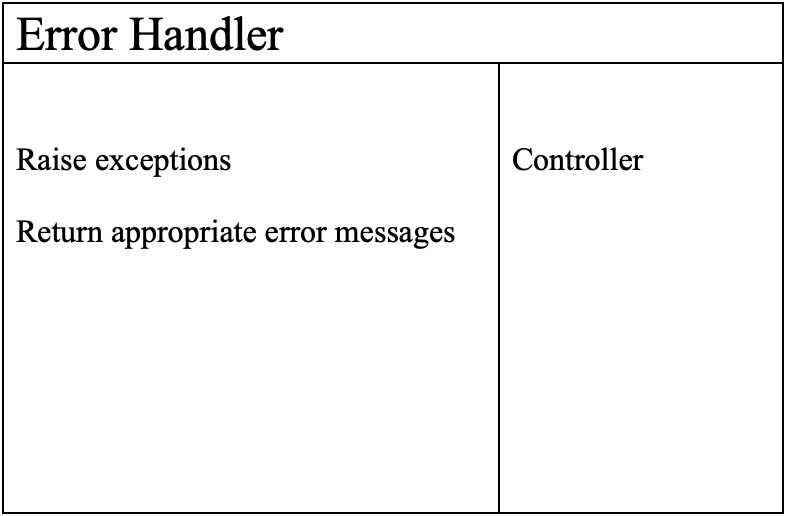
\includegraphics[width=.3\linewidth]{resources/ErrorHandler.png} 
            \hspace*{30pt}
          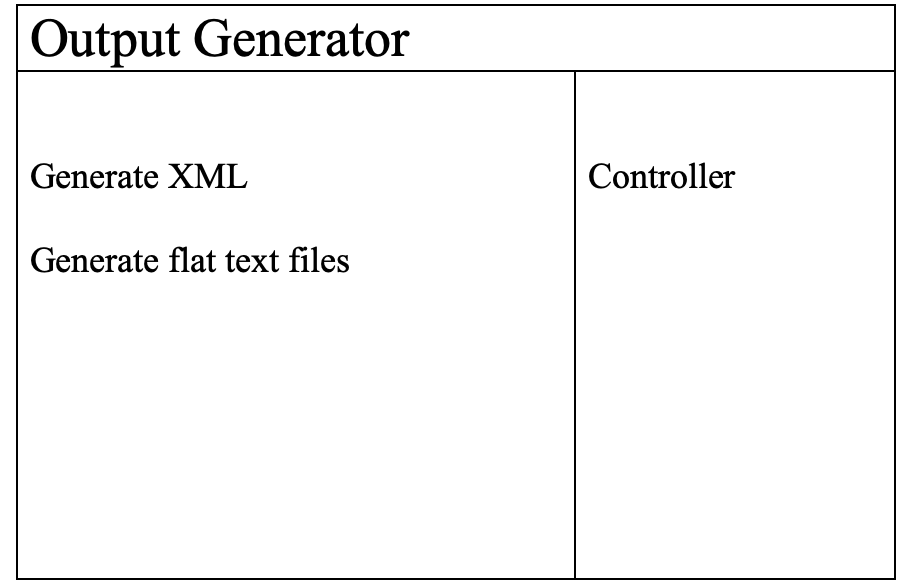
\includegraphics[width=.3\linewidth]{resources/OutputGenerator.png}
        \end{tabular}
        
        \begin{tabular}{@{}c@{}}
          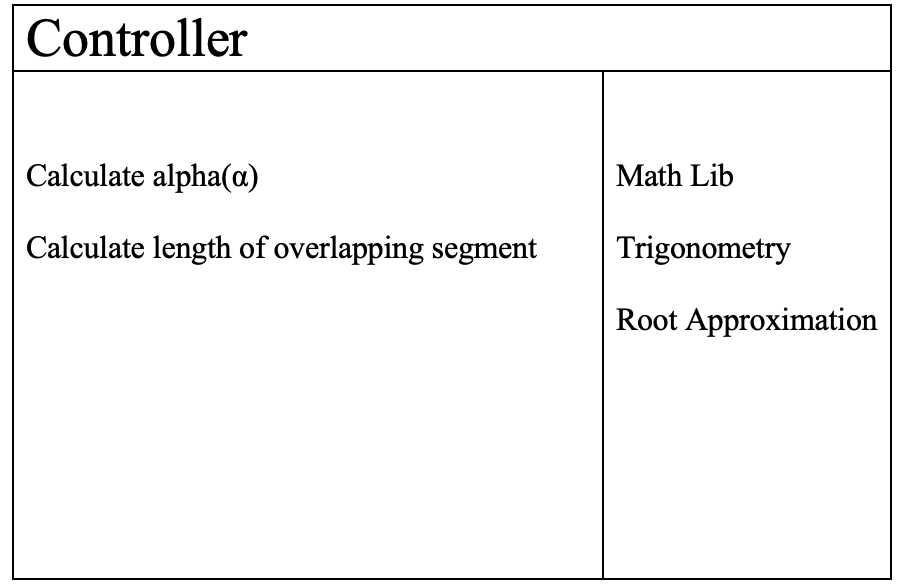
\includegraphics[width=.4\linewidth,height=90pt]{resources/Controller.png}
        \end{tabular}

        \vspace{\floatsep}
      \caption{CRC Cards for CHEERS}\label{fig:myfig}
  \end{figure}
